\documentclass[10pt,a4paper]{article}
\usepackage[a4paper,margin=18mm,top=18mm,bottom=18mm]{geometry}
\usepackage[T1]{fontenc}
\usepackage[utf8]{inputenc}
\usepackage{lmodern,microtype}
\usepackage[table]{xcolor}
\usepackage{booktabs,longtable,tabularx,array,ragged2e}
\usepackage{enumitem}
\usepackage{amssymb}
\usepackage{csquotes}
\usepackage{tikz}
\usepackage{pgfplots}
\pgfplotsset{compat=1.18}
\usetikzlibrary{positioning,arrows.meta}
\usepackage{fancyhdr,titlesec}
\usepackage[colorlinks=true,linkcolor=blue!60!black,citecolor=blue!60!black,urlcolor=blue!60!black]{hyperref}
\usepackage[backend=biber,style=ieee,sorting=none,maxnames=5]{biblatex}
\addbibresource{RTC_2027_3km_Avionics_SLR_Corrected.bib}
\definecolor{navy}{HTML}{18344F}
\definecolor{teal}{HTML}{087B80}
\definecolor{pale}{HTML}{EEF4F7}
\definecolor{graytext}{HTML}{55616D}
\newcolumntype{L}[1]{>{\RaggedRight\arraybackslash}p{#1}}
\newcolumntype{Y}{>{\RaggedRight\arraybackslash}X}
\setlength{\parindent}{0pt}
\setlength{\parskip}{4pt}
\setlength{\emergencystretch}{2em}
\setlength{\tabcolsep}{4pt}
\renewcommand{\arraystretch}{1.13}
\setlist[itemize]{leftmargin=1.4em,itemsep=2pt,topsep=2pt}
\setlist[enumerate]{leftmargin=1.4em,itemsep=2pt,topsep=2pt}
\titleformat{\section}{\large\bfseries\color{navy}}{\thesection}{.5em}{}
\titleformat{\subsection}{\normalsize\bfseries\color{teal}}{\thesubsection}{.5em}{}
\pagestyle{fancy}\fancyhf{}
\fancyhead[L]{\scriptsize RTC 2027 | 3 km avionics evidence review}
\fancyhead[R]{\scriptsize 4 November 2026}
\fancyfoot[C]{\scriptsize\thepage}
\renewcommand{\headrulewidth}{.3pt}
\hypersetup{pdftitle={Systematic Evidence Review of Avionics in Student Rocket Competitions at or around 3 km Apogee}}
\begin{document}
\begin{center}
{\small\bfseries\color{teal}LITERATURE EVIDENCE REPORT --- REPRODUCIBLE RAPID SCOPING REVIEW}\\[4pt]
{\LARGE\bfseries\color{navy}Avionics Systems in Student Rocket Competitions}\\[3pt]
{\large Near 3 km apogee: 3K and 10,000-ft student competition classes}\\[5pt]
{\small Evidence to inform the RTC 2027 Student 3K Mission Design Report (MDR)}\\[2pt]
{\small Search and verification cut-off: 4 November 2026}
\end{center}
\vspace{1mm}\hrule\vspace{3mm}

\begin{abstract}
\noindent\textbf{Objective.} Identify documented flight computers, sensors, telemetry, recovery electronics and validation practices in student competition rockets within a measured or nominal 3-km apogee class, and map that evidence to RTC 2027 MDR claims. \textbf{Search.} The user's first broad Web of Science Topic strategy combined rocket/launch-vehicle/missile terms with avionics, navigation and telemetry terms; exports were labelled 1609 Web of Science and 788 IEEE Xplore records. \textbf{Methods.} The unique supplied files contained 2396 parsable BibTeX records (1609 WOS and 787 IEEE); 75 DOI/title duplicates were removed, leaving 2321 unique records. A documented broad title/abstract filter yielded 1148 candidates; 121 met a prioritisation score. Supplementary student-team technical reports and theses were also identified. \textbf{Results.} Seven competition/competition-linked examples and six contextual avionics sources were examined. Published AVES II design data document duplicated pressure, inertial, GNSS and storage components, but the available evidence does not establish superiority of a Raspberry Pi Pico system. Graphs show the screening profile, bibliographic topic signals, evidence classes and a primary reported hardware inventory; a separate battery curve is clearly labelled as an engineering model. \textbf{Limitations.} This is a rapid systematic \emph{scoping} review, not a completed PRISMA systematic review: most candidates were not independently full-text screened, and nominal target altitude is not necessarily achieved apogee. \textbf{Conclusion.} The evidence supports a modular sensing, logging and redundant-recovery design \emph{concept}, while actual Pico flight readiness must be established through simulation and test.
\end{abstract}

\section{Review question and scope}
\textbf{Question:} What flight computers, sensors, telemetry, data storage, electrical power and recovery-control arrangements have been documented in student rocketry competitions with nominal apogees at or near 3 km, and what validation evidence exists for their use?

\textbf{Apogee eligibility is explicitly classified:} \textbf{A} = measured apogee $\leq3000$ m; \textbf{B} = nominal 3000 m competition class (actual flight apogee unspecified); \textbf{C} = a documented lower-altitude competition (actual individual flight apogee unknown); and \textbf{D} = relevant sounding-rocket research lacking sufficient altitude or competition evidence, retained only for contextual synthesis. In the 2026/2027 RTC ``3K'' category, the nominal goal is at least 3 km; that categorisation does not imply every entry's actual apogee was exactly or below 3000 m \cite{rtc2027rules}. We include the 10,000-ft (3048-m) IREC class as a \emph{near-3-km adjacent competition stratum}, not as a measured apogee $\le3000$ m.


\section{Methods}
\subsection{Review design, eligibility and research questions}
This is a \emph{rapid, systematic scoping evidence review}, not a completed two-reviewer systematic review or meta-analysis. It asks which flight computers, sensors, recovery-control arrangements, power systems, data logging and telemetry architectures were \emph{documented} for student competition rockets whose nominal class or measured apogee is at or near 3 km. A further question is which directly documented design features can support RTC 2027 MDR requirements, rather than which commercial board is ``best.'' The review uses PRISMA 2020 and PRISMA-S as \emph{reporting guidance}, while disclosing incomplete screening and the absence of a prospectively registered protocol \cite{page2021,rethlefsen2021}.

\textbf{Eligibility.} Include as primary evidence: a named student competition/team, a measured flight altitude $\leq3000$ m, credible nominal 3-km class, documented lower-altitude event, or a 10,000-ft adjacent class, and at least one citable avionics design feature or outcome. Class A: measured flight $\leq3000$ m; B: nominal 3-km class with unconfirmed measured apogee; C: documented lower-altitude competition context; D: informative rocketry research without the required competition/altitude link (context only). Class E is an adjacent 10,000-ft (3048-m) IREC target category, which is only 1.6\% above 3 km and is analysed separately, never relabelled as a $\le3000$-m flight. Preflight technical reports are not proof of flight success. Exclude from primary cases orbital launchers, general military missiles, unrelated aircraft/UAV systems, and avionics papers with no competition/altitude evidence.

\subsection{First search: databases, exact strategy and export counts}
The \textbf{first supplied search} was deliberately sensitive and broad; the original Web of Science Topic expression is reproduced verbatim below (line breaks added only for typesetting):
\begin{quote}\small\ttfamily
TS=((rocket* OR "launch vehicle*" OR "sounding rocket*" OR missile*)\newline
AND (avionics OR "flight computer*" OR "guidance system*"\newline
OR "navigation system*" OR "flight control system*"\newline
OR telemetry OR "attitude determination"))
\end{quote}
This initial search yielded the user's stated \textbf{1609 Web of Science} and \textbf{788 IEEE Xplore} records. The field tag \texttt{TS=} belongs to Web of Science; the precise IEEE Xplore interface-specific field translation/limits were \emph{not preserved} in the uploaded metadata, so no exact IEEE query is invented here. These counts are database-search \emph{labels}, not assertions that every record pertains to competition rocketry. The Web of Science export carries 3 November 2026 retrieval metadata; the IEEE export is labelled as the November 2026 collection. No unrecorded date/language limits are presumed. A complete future review should also search Scopus, aerospace conference repositories, EuRoC and IREC team reports, university theses and official competition reports with a separate competition-specific strategy. Such additional retrieval has not been counted as part of the original database-search totals.

\subsection{Bibliographic processing and transparent screening}
Three uploaded files were inspected: \texttt{Combined 1609.bib}, \texttt{Combined IEEE 788.bib} and \texttt{Combined IEEE 788(1).bib}. The two IEEE files have identical SHA-256 hashes, so only one was processed. The Web of Science file contains 1609 parsable entry starts; the IEEE file contains \textbf{787 actual BibTeX entry starts} despite ``788'' in its filename (a further \texttt{@} is part of a conference title). The processing sample is thus $1609+787=\mathbf{2396}$ parsed records. Titles, abstracts, source labels, year and DOI were extracted. Deduplication preferentially used normalised DOI, otherwise a lower-case, punctuation-stripped title. This removed \textbf{75} records and retained \textbf{2321} unique bibliographic records.

The post-export \emph{computational broad-screen proxy} required both a rocket-related expression and an electronics-related expression within combined title and abstract fields. The exact case-insensitive Python regular expressions are archived in the accompanying screening script; the term stems are also shown below.
\begin{quote}\footnotesize
\textbf{Rocket set:} rocket, sounding, launch vehicle, IREC, EuRoC, TEKNOFEST, spaceport.\\
\textbf{Electronics set:} avionics, flight computer, electronics, telemetry, data logging, parachute, recovery, apogee, flight control, sensor, attitude, control system, navigation, payload, onboard, embedded, altimeter, GPS, tracking.
\end{quote} Exactly \textbf{1148} matched; \textbf{1173} were non-matches. Among matches, an additive metadata heuristic (3 points for competition/student keywords in the title, 2 for avionics-related title terms, 2 for competition keywords in the abstract, 2 for altitude/apogee mentions in combined title/abstract; score threshold $\ge5$ of 9 possible points) identified \textbf{121 higher-priority candidates} (score $\geq5$). \textbf{This was not a comprehensive full-text screening of 121 studies}; the remaining 1027 broad candidates were not individually assessed in full.

Primary competition reports and institutional theses/webpages were additionally found through targeted searches and explicitly labelled as \emph{supplementary sources}, not silently counted inside the 2321 indexed records. Seven competition or competition-linked cases were extracted for the descriptive evidence table; six further studies were retained as secondary contextual evidence. The seven are not the final included sample from a complete PRISMA screening, nor evidence of the population prevalence of any hardware model.

\subsection{Data extraction, figure coding and appraisal}
The extraction fields were source/venue, competition, nominal versus measured apogee, MCU, inertial/pressure sensing, telemetry/GNSS, persistent data storage, recovery path, available testing/outcome evidence and limitations. Reliability class \textbf{R1} denotes a primary technical report or thesis, \textbf{R2} an experimental/HIL research paper, \textbf{R3} an institutional story, and \textbf{R4} abstract-only metadata. Inconsistently reported or absent items were treated as \emph{not disclosed}, not as absent hardware. No estimates of failure rates or processor ``win rates'' were made.

All graphs report their denominator and evidence basis. Workflow and year counts come from the two unique metadata exports. Figure~\ref{fig:topics} counts \emph{non-mutually-exclusive regular-expression signals}, not confirmed use of components in flight, and may include military/large launch-vehicle papers because the first search explicitly included \texttt{missile*}. Figure~\ref{fig:classes} summarises only the seven manually extracted competition cases. Figure~\ref{fig:aves2} uses an identifiable published component inventory in the \emph{AVES II} technical report. A separate analytic power model (Fig.~\ref{fig:power}) is marked as \emph{calculated engineering assumption}, not a flight measurement or an outcome extracted from the review \cite{astg2022aves2,rpicopico,rtc2027rules}.

\subsection{Reproducibility and departures from a complete SLR}
The accompanying package contains a screening script, the source-record audit and figure data tables (CSV). To independently reproduce the initial numbers, use the \emph{original} two BibTeX exports: the ZIP does not redistribute those large, user-supplied libraries. The included seven-case charts describe the original core sample; additional targeted 10,000-ft examples below are NOT part of that seven-case denominator. The current narrative/graphs represent an honest rapid evidence review; a journal-grade systematic review would require independently screened full texts for all potentially eligible records, exclusion reasons, search-platform settings, a registered protocol or predeclared amendments, and a completed PRISMA flow \cite{page2021,rethlefsen2021}.

\subsection{Search and screening profile (PGFPlots)}
\begin{figure}[htbp]\centering
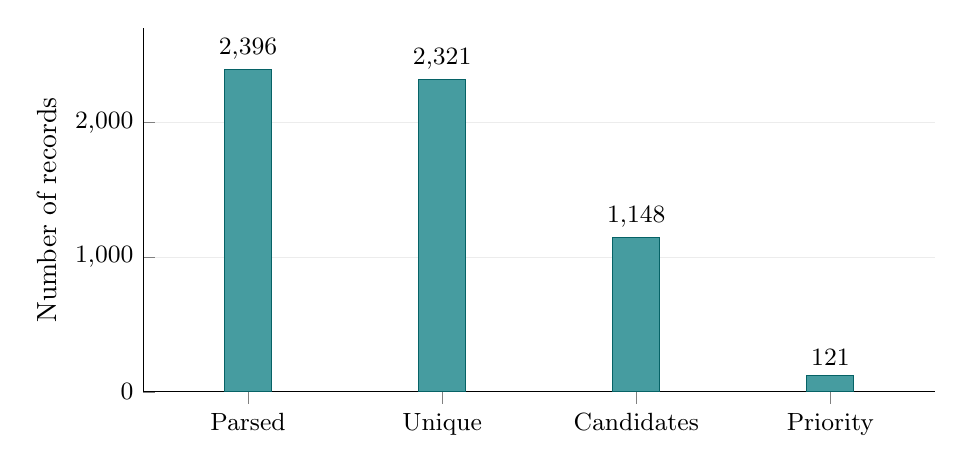
\begin{tikzpicture}
\begin{axis}[ybar,bar width=17pt,width=.96\linewidth,height=6.2cm,
  symbolic x coords={Parsed,Unique,Candidates,Priority},xtick=data,
  ylabel={Number of records},ymin=0,ymax=2700,
  nodes near coords,nodes near coords align={vertical},
  every node near coord/.append style={font=\small},
  enlarge x limits=.18,axis x line*=bottom,axis y line*=left,
  ymajorgrids,grid style={gray!15},tick label style={font=\small}]
\addplot[fill=teal!75,draw=teal!80!black] coordinates
  {(Parsed,2396) (Unique,2321) (Candidates,1148) (Priority,121)};
\end{axis}
\end{tikzpicture}
\caption{Sequential \emph{metadata-screening stages}: parsed records, DOI/title-deduplicated records, broad keyword candidates, and heuristic-priority candidates. The last bar is \emph{not} a full-text inclusion count. Data: exported bibliography and reproducible script.}
\label{fig:screening}
\end{figure}

\begin{figure}[htbp]\centering
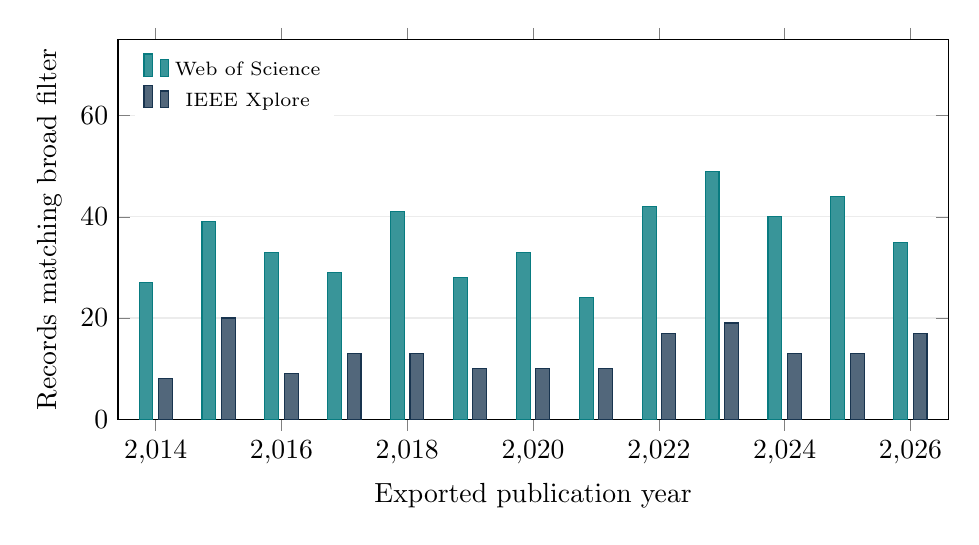
\begin{tikzpicture}
\begin{axis}[ybar,bar width=5pt,width=\linewidth,height=6.4cm,
  xlabel={Exported publication year},ylabel={Records matching broad filter},
  xmin=2013.4,xmax=2026.6,ymin=0,ymax=75,
  xtick={2014,2016,2018,2020,2022,2024,2026},
  legend style={at={(.02,.98)},anchor=north west,font=\scriptsize,draw=none,fill=white},
  ymajorgrids,grid style={gray!15}]
\addplot[fill=teal!80,draw=teal] coordinates {
(2014,27) (2015,39) (2016,33) (2017,29) (2018,41) (2019,28) (2020,33) (2021,24) (2022,42) (2023,49) (2024,40) (2025,44) (2026,35)
};
\addlegendentry{Web of Science}
\addplot[fill=navy!75,draw=navy] coordinates {
(2014,8) (2015,20) (2016,9) (2017,13) (2018,13) (2019,10) (2020,10) (2021,10) (2022,17) (2023,19) (2024,13) (2025,13) (2026,17)
};
\addlegendentry{IEEE Xplore}
\end{axis}
\end{tikzpicture}
\caption{Publication-year distribution for the \emph{636 of 1148 keyword-filtered records dated 2014--2026}, by retained source; records outside this window are not plotted. This shows the broad initial literature landscape and \emph{does not} estimate the number of qualifying 3-km student flights. Data: \texttt{figure\_annual\_counts.csv}.}
\label{fig:annual}
\end{figure}

\begin{figure}[htbp]\centering
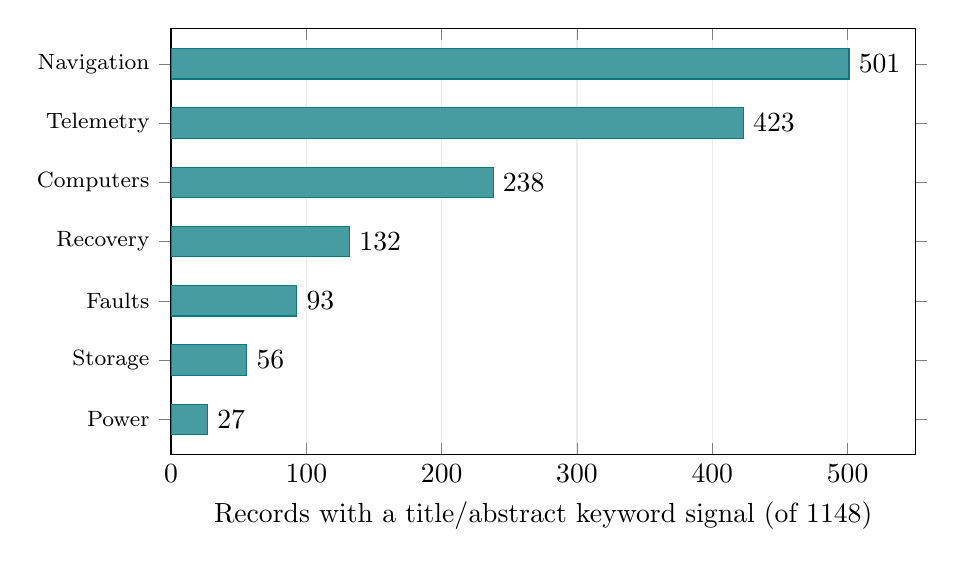
\begin{tikzpicture}
\begin{axis}[xbar,width=.91\linewidth,height=7cm,xmin=0,xmax=550,
  symbolic y coords={Power,Storage,Faults,Recovery,Computers,Telemetry,Navigation},
  ytick=data,yticklabel style={font=\footnotesize},
  xlabel={Records with a title/abstract keyword signal (of 1148)},
  nodes near coords,nodes near coords align={horizontal},
  enlarge y limits=.1,bar width=11pt,
  xmajorgrids,grid style={gray!15}]
\addplot[fill=teal!75,draw=teal] coordinates {
 (27,Power) (56,Storage) (93,Faults) (132,Recovery)
 (238,Computers) (423,Telemetry) (501,Navigation)
};
\end{axis}
\end{tikzpicture}
\caption{\emph{Non-exclusive lexical signals} in the 1148 broad candidates: navigation/IMU/barometric/GPS (501), telemetry (423), flight computer/avionics (238), recovery/deployment (132), fault tolerance/redundancy (93), storage/logging (56), power/energy (27). Counts use documented regular expressions, not actual installed-hardware frequencies.}
\label{fig:topics}
\end{figure}

\section{Results: competition cases inside or nominally at 3 km}
\small
\begin{longtable}{@{}L{30mm}L{22mm}L{51mm}L{39mm}@{}}
\toprule\rowcolor{pale}\textbf{Team / source} & \textbf{Apogee eligibility} & \textbf{Documented avionics hardware and functions} & \textbf{Evidence / limitations}\\\midrule\endfirsthead
\toprule\rowcolor{pale}\textbf{Team / source} & \textbf{Altitude} & \textbf{Avionics evidence (continued)} & \textbf{Limitations}\\\midrule\endhead
\bottomrule\endlastfoot
ASTG \emph{AVES} (EuRoC 2021) \cite{astg2021aves} & B: 3000-m target class & Custom dual-core ARM flight computer; 6-DOF IMU, separate high-g accelerometer, barometer, two GNSS receivers, SD and flash memory, RavenOS, telemetry; COTS flight-computer path and two-stage recovery. & R1 team technical report; 3000 m is the mission target, not independently verified recorded apogee.\\
ASTG \emph{AVES II} (EuRoC 2022) \cite{astg2022aves2} & B: 3000-m target class & STM32H745ZI (Cortex-M7/M4), custom flight computer and RTOS RavenOS, telemetry, sensor redundancy, black box/cameras; SRAD and COTS recovery-control paths; Eggtimer Quantum used for official logging rather than redundant recovery. & R1 detailed pre-flight technical report including ground-test annexes; team reports a completed EuRoC flight, but numeric flight apogee is not established here.\\
CTU \emph{ILLUSTRIA} flight-computer study (2024) \cite{zlamala2024} & B: linked to nominal 3-km EuRoC entry & Custom STM32H743 board; pressure/inertial sensing, CAN/SPI/I$^2$C, PX4/NuttX state machine, MAVLink and software-/hardware-in-loop methodology. & R1 university thesis; bench/HIL design validation, not proof the same board completed a 3-km flight.\\
Zapadlo's 2023 Czech Rocket Challenge computer \cite{zapadlo2023,czech2026} & C: lower-altitude event (organiser presently lists 400--800 m typical) & STM32 flight computer with LoRa; battery/supercapacitor selector, redundant-power design and telemetry. & R4 repository abstract; verified on stratospheric balloon, not asserted as rocket flight-proven. 2026 category figures used as approximate context only.\\
Kadlec and Walla model-rocket project (Czech Rocket Challenge experience) \cite{kadlec2024,czech2026} & C: lower-altitude competition context & Barometric altitude, acceleration, attitude, temperature and GNSS; onboard logging, image capture, real-time ground communication and autonomous operation after link loss. & R1 published student proceedings; specific project apogee and detailed microcontroller not established from reviewed portions.\\
Tamkang \emph{Stargazer} demonstration at RTC 2026 \cite{stargazer2026} & A: reported 2956 m measured & New-generation avionics were tested on the demonstration flight; organisers' motor used. & R3 institutional news report; genuine altitude/outcome, but no published sensor/MCU list in source. Not presented as a competing finalist.\\
National Formosa University \emph{Skybound Singularity}, RTC 2026 \cite{nfu2026} & B: RTC Student 3K category & Recovery and payload deployment featured in the mission; electronic system detail and individual MCU/sensor models not substantiated by this source. & R3 university results report; 3K category and award confirmed; exact apogee and full avionics bill unavailable.\\
\end{longtable}
\normalsize


\subsection{Evidence coverage and a directly documented hardware example}
\begin{figure}[htbp]\centering
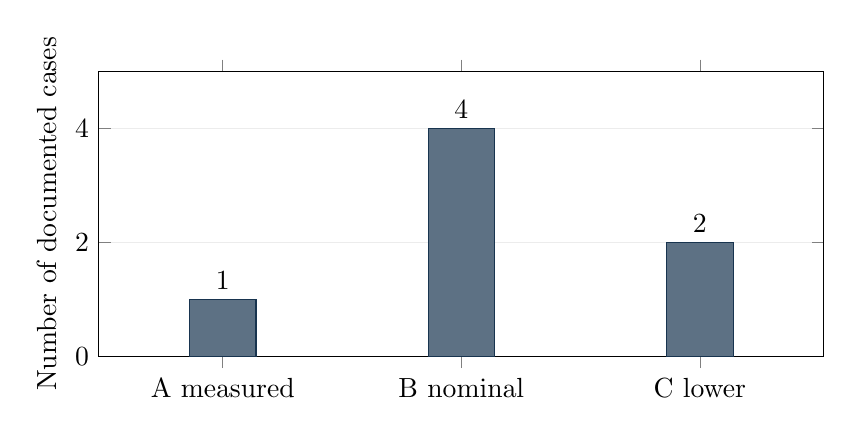
\begin{tikzpicture}
\begin{axis}[ybar,width=.89\linewidth,height=5.2cm,ymin=0,ymax=5,
 symbolic x coords={A measured,B nominal,C lower},xtick=data,
 ylabel={Number of documented cases},
 nodes near coords,bar width=24pt,
 ymajorgrids,grid style={gray!15},enlarge x limits=.26]
\addplot[fill=navy!70,draw=navy] coordinates {(A measured,1) (B nominal,4) (C lower,2)};
\end{axis}
\end{tikzpicture}
\caption{Eligibility status of the \emph{seven manually extracted competition/competition-linked examples}. Only one has a published measured apogee within 3 km (Tamkang's demonstration); four are nominal 3-km-class projects, and two are lower-altitude competition-linked projects. No prevalence, reliability or success-rate inference is warranted \cite{stargazer2026,astg2021aves,astg2022aves2,zlamala2024,nfu2026,zapadlo2023,kadlec2024}.}
\label{fig:classes}
\end{figure}

\begin{figure}[htbp]\centering
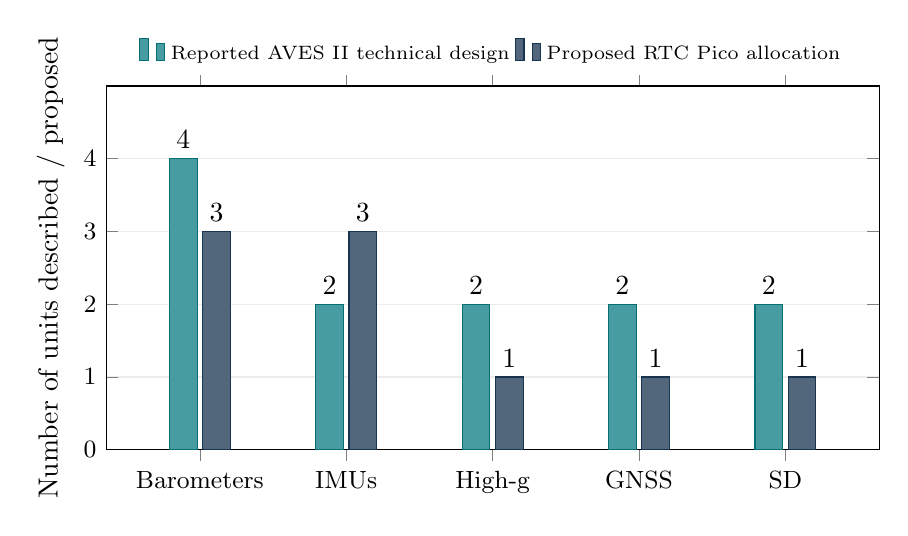
\begin{tikzpicture}
\begin{axis}[ybar,width=.94\linewidth,height=6.2cm,ymin=0,ymax=5,
 symbolic x coords={Barometers,IMUs,High-g,GNSS,SD},xtick=data,
 ylabel={Number of units described / proposed},
 ytick={0,1,2,3,4},ymajorgrids,grid style={gray!15},
 enlarge x limits=.16,bar width=10pt, nodes near coords,
 legend style={at={(.5,1.03)},anchor=south,legend columns=2,font=\scriptsize,draw=none},
 tick label style={font=\small}]
\addplot[fill=teal!75,draw=teal!90!black] coordinates
 {(Barometers,4)(IMUs,2)(High-g,2)(GNSS,2)(SD,2)};
\addlegendentry{Reported AVES II technical design}
\addplot[fill=navy!75,draw=navy] coordinates
 {(Barometers,3)(IMUs,3)(High-g,1)(GNSS,1)(SD,1)};
\addlegendentry{Proposed RTC Pico allocation}
\end{axis}\end{tikzpicture}
\caption{\textbf{Descriptive design comparison, not performance evidence.} AVES II's published preflight inventory reports 2 BMP390 plus 2 MS5607 barometers (4 total), 2 BMI088 IMUs, 2 H3LIS331DL high-g sensors, 2 SAM-M8Q GNSS receivers, and 2 SD cards \cite{astg2022aves2}. The proposed RTC allocation includes 3 barometers, 3 MPU6050 IMUs, 1 baseline ADXL375 high-g sensor, 1 organiser GPS beacon and 1 logger SD; this proposal is \emph{unqualified}, with separate FRAM checkpoints excluded from the SD count. Counts describe architecture only; higher counts do not establish greater reliability.}
\label{fig:aves2}
\end{figure}

\subsection{Interpreting the primary competition evidence}
\textbf{Convergent functions:} (i) pressure and inertial sensing for flight phase recognition; (ii) logging independent of ground communications; (iii) parachute deployment control separated from at least some non-safety subsystems; (iv) telemetry or GPS for recovery and post-flight analysis; (v) explicit ground or simulation verification. The best documented 3-km team reports are AVES and AVES II; this is not evidence that their exact parts are universally optimal \cite{astg2021aves,astg2022aves2}.

\textbf{Architectural diversity:} 3-km AVES II uses a custom high-performance STM32 MCU plus separate COTS electronics; the Czech challenge thesis documents an STM32-plus-supercapacitor arrangement; the RTC Stargazer report demonstrates an actual near-3-km flight but does not expose its part numbers. Consequently, there is no defensible numerical frequency table of microcontroller brands for all 3-km competition finalists \cite{astg2022aves2,zapadlo2023,stargazer2026}.

\section{Contextual avionics research: altitude or competition unverified}
These studies appeared in, or are strongly linked to, the uploaded literature libraries. They \emph{support engineering reasoning} but were \emph{not included as verified $\leq3$-km competition flight cases}.
\small
\begin{longtable}{@{}L{45mm}L{69mm}L{28mm}@{}}
\toprule\rowcolor{pale}\textbf{Study} & \textbf{Relevant evidence} & \textbf{Why secondary}\\\midrule\endfirsthead
\toprule\rowcolor{pale}\textbf{Study} & \textbf{Evidence} & \textbf{Reason}\\\midrule\endhead
\bottomrule\endlastfoot
Netzel et al. (2026), \emph{HardwareX} \cite{netzel2026} & STM32F407, high-g ADXL375, IMU, MS5607 barometer and non-volatile logging, with end-to-end hardware-in-the-loop (HIL) phase/event testing. & No demonstrated competition flight; published HIL study.\\
Pathak et al. (2022), S3FC \cite{pathak2022} & Launch interlocks, filtering against false deployment, GPS downlink and CRC for telemetry integrity. & Exact apogee/category absent in available abstract.\\
Kahe (2017) \cite{kahe2017} & COTS-based dual-redundant sounding-rocket flight computer. & No verified 3-km competition altitude.\\
Moschidis and Bithas (2022) \cite{moschidis2022} & Model rocket using accessible Arduino flight-computer components and simulation-to-flight comparison. & Specific student competition and target apogee unverified.\\
Bakirci and Ozer (2022) \cite{bakirci2022} & Scientific experiment unit integrated with subsonic rocket avionics, telemetry and recovery functions. & Competition/apogee linkage unverified.\\
Andrade et al. (2022) \cite{andrade2022} & Heltec LoRa 32 proof-of-concept sounding-rocket telemetry. & Proof of concept; no verified competition flight at $\leq3$ km.\\
\end{longtable}
\normalsize

\section{Evidence synthesis by avionics subsystem}
\small
\begin{longtable}{@{}L{31mm}L{72mm}L{39mm}@{}}
\toprule\rowcolor{pale}\textbf{Subsystem} & \textbf{Finding from case studies} & \textbf{RTC 2027 implication}\\\midrule\endfirsthead
\toprule\rowcolor{pale}\textbf{Subsystem} & \textbf{Finding} & \textbf{MDR implication}\\\midrule\endhead
\bottomrule\endlastfoot
Flight computer & Primary 3-km reports favour purpose-built MCU-based computers; STM32 explicitly documented in AVES II and ILLUSTRIA. Other lower-altitude designs use STM32/LoRa; selected small-model research uses Arduino. \cite{astg2022aves2,zlamala2024,zapadlo2023,moschidis2022} & Pico is a \emph{candidate}, not literature-proven best choice; compare compute/I/O, power, failure modes, software support and qualification tests.\\
Altitude / motion & Inertial + barometric sensors occur repeatedly; AVES documents a separate high-g accelerometer, an important precedent for full boost-range logging. \cite{astg2021aves,netzel2026} & Validate MPU6050 $\pm16g$ against actual thrust/mass/shock envelope; specify barometer venting and sensor error handling.\\
Data logging & Local SD/flash or black-box recording decouples mission evidence from an intermittent radio link. \cite{astg2021aves,astg2022aves2,netzel2026} & Propose timestamped non-volatile flight record; demonstrate buffer occupancy and recoverable data after resets.\\
Recovery / redundancy & AVES II includes separate custom and commercial flight-computer paths; lower-altitude work examines alternate power sources. \cite{astg2022aves2,zapadlo2023} & Redundant Picos are an unvalidated \emph{team design}; scrutinise common-mode firmware, barometer/pressure port and shared release mechanism failures.\\
Telemetry and position & Team implementations range from custom ground stations to LoRa, while RTC requires its standard GPS beacon. \cite{astg2021aves,zapadlo2023,andrade2022,rtc2027rules} & Mandatory official GPS cannot be replaced with an unapproved radio; extra telemetry requires frequency compliance.\\
Testing & EuRoC technical reports include subsystem ground-test evidence; ILLUSTRIA and Netzel demonstrate simulation/HIL methods. \cite{astg2022aves2,zlamala2024,netzel2026} & Include pressure/flight-profile replay, safe recovery test loads, battery endurance, vibration, data integrity and integration testing in MDR verification plan.\\
\end{longtable}
\normalsize

\section{Implications for the Raspberry Pi Pico MDR concept}
The present team proposes one Raspberry Pi Pico as a non-safety logger/payload computer and two additional, independently powered controllers as potential recovery channels. This architecture is not claimed to have appeared in a verified 3-km competition report. Its justification should instead be written as a \emph{traceable engineering proposal}: low MCU cost and I/O capability \cite{rpicopico}; precedent for separate mission and recovery duties \cite{astg2022aves2}; and documented need for deterministic event handling and HIL testing \cite{netzel2026}. The final recovery arrangement must meet the specific 2027 RTC release and arming rules \cite{rtc2027rules}.

\begin{tabularx}{\linewidth}{@{}L{32mm}Y L{45mm}@{}}
\toprule\rowcolor{pale}\textbf{Decision} & \textbf{Evidence-supported rationale} & \textbf{Evidence still needed}\\\midrule
Pico for logger & Low-cost, open ecosystem; separate acquisition and storage tasks can be implemented and benchmarked \cite{rpicopico}. & Measured sample jitter, storage stalls and energy use with production hardware.\\
IMU + barometer & Similar measurement functions appear in published competition systems \cite{astg2021aves,astg2022aves2}. & Peak-g simulation, pressure-port bias and calibration error.\\
Recovery A/B & Comparable reports use distinct recovery-computer paths \cite{astg2022aves2}. & Independent release-device feasibility, common-cause FMEA and repeated safe-load tests.\\
Local logs + GPS & Black-box data preservation is a documented approach \cite{astg2021aves,netzel2026}. & Retrieved official beacon data, timestamp alignment and storage integrity.\\
Payload acquisition & Experimental payload and rocket avionics can be integrated as a separate function \cite{astg2021aves,bakirci2022}. & Declared scientific objective, calibration and measurable flight success criteria.\\
\bottomrule
\end{tabularx}


\subsection{Quantitative engineering check: proposed logger power and storage (model, not flight evidence)}
The reviewed competition studies support the \emph{architecture and functions}, not a numerical Pico endurance guarantee. To make the RTC electrical-endurance claim testable, a separate, explicitly \emph{assumption-based} preliminary model uses a nominal 3.7-V, 2.6-Ah cell ($9.62$ Wh), $85\%$ converter efficiency, and $3.3$-V subsystem operating voltage. With a constant average current $I$ (amperes), predicted runtime is
\[
 t_{\mathrm{ideal}}(I)=\frac{3.7\,(2.6)\,(0.85)}{3.3\,I}\;\mathrm{hours}.
\]
The team design proposal assumes an average logger load near 56 mA but conservatively sizes around 200 mA; the predicted duration at 200 mA is about 12.39 h. This \emph{is not a measured runtime}: battery capacity derating, cut-off voltage, peak SD-card write current, protection losses, temperature, ageing and release loads must be tested. The RTC's $>1.5$ h requirement applies to the actual assembled system \cite{rtc2027rules,rpicopico}.

\begin{figure}[htbp]\centering
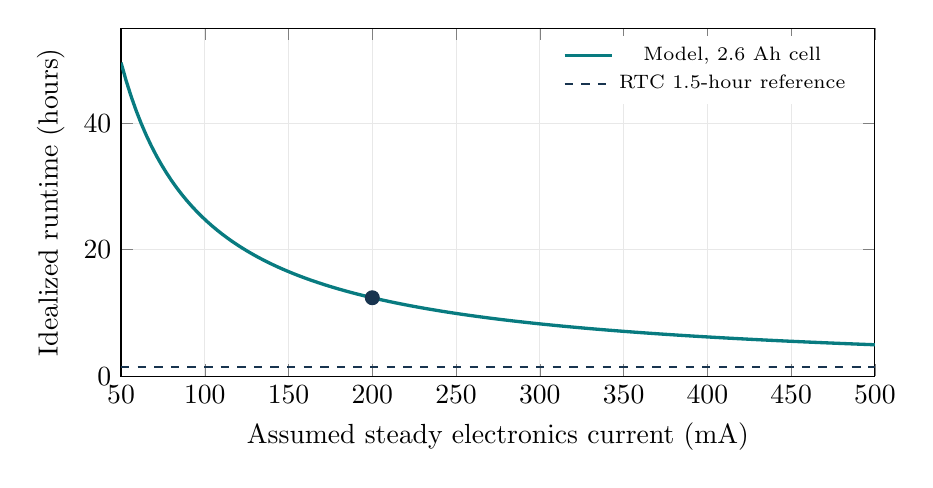
\begin{tikzpicture}
\begin{axis}[width=.92\linewidth,height=6cm,
 xmin=50,xmax=500,ymin=0,ymax=55,
 xlabel={Assumed steady electronics current (mA)},ylabel={Idealized runtime (hours)},
 domain=50:500,samples=150,
 grid=major,grid style={gray!18},
 legend style={at={(.98,.98)},anchor=north east,font=\scriptsize,draw=none}]
\addplot[teal,very thick]{3.7*2.6*0.85/(3.3*(x/1000))};
\addlegendentry{Model, 2.6 Ah cell}
\addplot[navy,dashed,thick,domain=50:500]{1.5};
\addlegendentry{RTC 1.5-hour reference}
\addplot[only marks,mark=*,mark size=2.5pt,navy] coordinates {(200,12.39)};
\end{axis}
\end{tikzpicture}
\caption{\textbf{Calculated scenario, not test results}. Predicted battery-endurance envelope for the proposed logger under stated assumptions. At 200 mA, predicted runtime is about 12.4 h; qualification still requires an actual $>1.5$ h endurance test \cite{rtc2027rules,rpicopico}.}
\label{fig:power}
\end{figure}

\textbf{Storage sizing (calculated).} The revised MDR proposes a 44-byte fixed record at 200 samples/s, including IMU, high-g and two temperature channels; this gives $44\times200=8800$ B/s; across 90 min, $47.52$ MB (decimal). This supports a preliminary memory-capacity choice, \emph{not} evidence that microSD write latency, vibration retention or file-system reliability meets flight requirements. The latter must be measured with a worst-case logging test.


\section{Adjacent 10,000-ft IREC competition stratum (3048 m)}
The 10,000-ft IREC category is an especially relevant comparator to RTC 3K because $10,000\,\mathrm{ft}\times0.3048=3048\,\mathrm{m}$, only 48 m (1.6\%) above a nominal 3,000 m target. To avoid changing the original seven-case descriptive figures without rerunning the complete search, this additional stratum is presented \emph{separately}, not added to Figures~\ref{fig:classes} or~\ref{fig:aves2}. The first broad indexed search lacked competition terms and was supplemented by team-project web reports, so neither figure should be treated as a comprehensive sample.

\textbf{River City Rocketry ``Sovereignty'' (2026 IREC 10k COTS):} the project description documents two commercial recovery electronics units (Blue Raven and StratologgerCF), independent GPS trackers (Featherweight and Telemetrum), locally recorded sensor data and a separate functional payload with its own power \cite{irec2026sovereignty}. The website reports a \emph{target} of 10,000 ft and a \emph{predicted} 10,618 ft, so it is a design comparator, not evidence of successful flight or a measured achieved apogee. It supports discussion of functional and power-domain separation, but the pyrotechnic architecture described by this US competition entry cannot be assumed compatible with RTC 2027.

\textbf{Implication for Pico MDR.} AVES/AVES II directly motivate separate high-g measurement and redundant recovery architectures; 10,000-ft IREC projects provide an additional comparison for independent commercial recovery electronics and GPS paths. None demonstrates that three Pico development boards have flight-qualified reliability; the current proposal still needs simulation and bench/qualification tests \cite{astg2021aves,astg2022aves2,irec2026sovereignty}.


\section{Suggested MDR requirement--evidence map}
\small
\begin{tabularx}{\linewidth}{@{}L{25mm}Y L{47mm}@{}}
\toprule\rowcolor{pale}\textbf{RTC topic} & \textbf{Relevant published precedent} & \textbf{Planned evidence for MDR/PDR}\\\midrule
Required flight data & AVES primary multi-sensor, logging and GNSS architecture \cite{astg2021aves}; RTC specification \cite{rtc2027rules}. & Data-flow diagram; rate/range table; bench data replay.\\
Drogue and main & AVES/AVES II two-stage recovery and redundant avionics \cite{astg2021aves,astg2022aves2}. & Proposed logic, two-path release diagram, fault analysis.\\
Power endurance & Alternate power-path design in lower-altitude competition thesis \cite{zapadlo2023}; RTC electrical rule \cite{rtc2027rules}. & Per-domain power budget, battery protections and endurance plan.\\
Mission payload & AVES student CanSats and ILLUSTRIA sensor integration \cite{astg2021aves,zlamala2024}. & Payload mission and measurable criteria; thermal calibration plan.\\
Verification & AVES II test appendices, ILLUSTRIA HIL thesis and Netzel et al. HIL \cite{astg2022aves2,zlamala2024,netzel2026}. & Planned hardware-in-loop, safe-load, vibration and data checks.\\
\bottomrule
\end{tabularx}
\normalsize


\section{Evidence-to-MDR claim audit: what the figures do and do not establish}
\small
\begin{longtable}{@{}L{31mm}L{57mm}L{55mm}@{}}
\toprule\rowcolor{pale}\textbf{MDR proposal} & \textbf{Directly documented supporting evidence} & \textbf{Proposed claim and unverified gap}\\\midrule\endfirsthead
\toprule\rowcolor{pale}\textbf{Proposal} & \textbf{Evidence (continued)} & \textbf{What is NOT proven}\\\midrule\endhead
\bottomrule\endlastfoot
Modular MCU flight computer & AVES II reports custom STM32H745ZI and distinct recovery/electronics functions; thesis documents STM32H743, software/HIL validation \cite{astg2022aves2,zlamala2024}. & Supports feasibility of the \emph{functional architecture}; no published verification of three Picos for an RTC 3K flight.\\
Barometer + IMU + high-g sensing & AVES II reports duplicate barometers/IMUs and high-g accelerometers (Fig.~\ref{fig:aves2}) \cite{astg2022aves2}. & Validate BMP280 pressure ports and whether MPU6050 $\pm16g$ clips during boost/deployment and whether a baseline $\pm200g$ ADXL375 is adequate; model is not a sensor qualification.\\
Independent recovery paths & AVES II documents SRAD/COTS functions and redundant sensor paths \cite{astg2022aves2}; separate technical source discusses redundancy \cite{kahe2017}. & Do not infer a recovery failure probability from team reports. Common pressure environments, firmware and mechanical release remain possible single-point failures.\\
Persistent flight data and GPS & AVES/AVES II describe flight-data storage, GNSS and telemetry \cite{astg2021aves,astg2022aves2}. & RTC official GPS beacon compatibility and access to the trajectory file remain team integration work.\\
Power $>1.5$ h and storage & Power curve (Fig.~\ref{fig:power}) and 47.52-MB revised storage need are conditional calculations; manufacturer Pico specification \cite{rpicopico}. & Not proof of real cell capacity, SD-card reliability, connector survival or launch loads. Full-power endurance and fault tests remain mandatory.\\
Payload experiment & Student payload integration is documented in AVES and experimental rocket studies \cite{astg2021aves,bakirci2022}. & The team's two-probe thermal mission still needs its own calibration, uncertainty analysis and measurable flight success criteria.\\
\end{longtable}
\normalsize

\section{Evidence quality, limitations and conclusions}
\textbf{Evidence quality.} Two team reports provide unusually rich 3-km detail but were prepared by the same organisation in successive years. One university thesis provides a 3-km design connection but not a verified flight of its new computer. Lower-altitude case studies are useful for power, telemetry and design development but operate in different loads and mission envelopes. A university news report gives actual near-3-km apogee with almost no reproducible avionics BOM. These weaknesses preclude a pooled success rate, failure probability or ranking of processors.

\textbf{Review limitations.} (1) A single reviewer applied the screening workflow; (2) 1027 broad candidate records were not all individually fully screened; (3) no protocol was prospectively registered; (4) publication and outcome reporting are highly variable; (5) multiple primary technical reports were published pre-flight, while flight outcomes appeared separately; (6) published web documentation can change; (7) nominal 3-km target is not the same as measured apogee $\leq3000$ m. To upgrade this work to a formal systematic review, independently screen all 2321 records (or a pre-registered refined search with documented exclusions), retrieve all eligible full texts, and provide a complete PRISMA flow and critical appraisal \cite{page2021,rethlefsen2021}.

\textbf{Conclusion.} Public evidence for approximately 3-km student competition avionics favours modular MCU-based design, calibrated barometric/inertial sensing, flight logging independent of telemetry, well-defined recovery redundancy and extensive ground verification. The evidence does \emph{not} establish any particular board as universally optimal. A Raspberry Pi Pico architecture can be defended in the RTC MDR as an economical preliminary design, provided the team specifies and eventually demonstrates its timing, sensor range, fault isolation, recovery authority, power margin and flight-data integrity against RTC requirements.

\printbibliography[title={References}]
\end{document}
